\section{Clase de un instrumento}

La clase de un instrumento es un indicador normalizado de su exactitud. Se define a partir del \textbf{error absoluto máximo} (\(E_\text{max}\)) que el instrumento puede cometer en cualquier punto de su escala, garantizado por el fabricante bajo condiciones normales de uso.

La clase (\(c\)) expresa este error máximo como un porcentaje del valor fiduciario (generalmente el alcance o fondo de escala):

\begin{equation}
    c = \frac{E_\text{max}}{X_\text{fid}} \cdot 100
    \label{eq:definicion_clase}
\end{equation}

Despejando esta ecuación, podemos conocer el límite de error en unidades de la magnitud medida (Voltios, Amperios, etc.) para cualquier lectura:

\[
    E_\text{max} = \pm \frac{c \cdot X_\text{fid}}{100}
\]

\begin{definition}[Valor Fiduciario (\(X_\text{fid}\))]
    Es el valor de referencia sobre el cual se calcula la clase.
    \begin{itemize}
        \item \textbf{Instrumentos con cero a la izquierda:} Coincide con el \emph{Alcance} (ej. Amperímetro \qtyrange{0}{100}{\ampere} \(\to X_\text{fid} = \qty{100}{\ampere}\)).
        \item \textbf{Instrumentos con cero central:} Es la suma de los valores absolutos de los límites (ej. Galvánometro \qtyrange{-15}{+15}{\milli\ampere} \(\to X_\text{fid} = \qty{30}{\milli\ampere}\)).
        \item \textbf{Instrumentos con cero suprimido:} Generalmente es el límite superior (ej. Voltímetro de red \qtyrange{180}{260}{\volt} \(\to X_\text{fid} = \qty{260}{\volt}\)).
    \end{itemize}
\end{definition}

\subsection{Interpretación y uso práctico}

En la práctica, desconocemos el error real en una medición específica. Adoptamos un criterio pesimista (o conservador): asumimos que en \emph{cualquier} punto de la escala estamos cometiendo el error máximo permitido por la clase.

\begin{example}
    Comparemos dos voltímetros midiendo una tensión real de \qty{10}{\volt}:
    \begin{itemize}
        \item \textbf{V1:} Alcance \qty{30}{\volt}, Clase 1.0.
        \item \textbf{V2:} Alcance \qty{30}{\volt}, Clase 0.2.
    \end{itemize}
    
    Los errores límites son:
    \[ E_{v1} = \pm \frac{1 \cdot 30}{100} = \pm \qty{0.3}{\volt} \quad ; \quad E_{v2} = \pm \frac{0.2 \cdot 30}{100} = \pm \qty{0.06}{\volt} \]
    
    Resultados de la medición:
    \begin{itemize}
        \item Con V1: \( 10 \pm \qty{0.3}{\volt} \) (Error relativo: \(3\%\)).
        \item Con V2: \( 10 \pm \qty{0.06}{\volt} \) (Error relativo: \(0.6\%\)).
    \end{itemize}
\end{example}

Los instrumentos de Clase 0.1 a 0.5 se reservan para laboratorio y calibración, mientras que los de Clase 1.0 a 2.5 (o mayores) se utilizan en tableros industriales donde la robustez es más importante que la extrema exactitud.

\subsection{Calibración y Verificación}

Para establecer la clase, el fabricante compara el instrumento contra un patrón de jerarquía superior bajo condiciones controladas (Temperatura \qtyrange{20}{25}{\degreeCelsius}, posición de trabajo especificada y ausencia de campos magnéticos externos\footnote{Menores a \qty{5}{\text{Oersted}} o aprox. \qty{400}{\ampere\per\meter}.}).

El proceso genera una \textbf{Curva de Corrección}: una gráfica que muestra la diferencia entre el valor leído y el valor real (patrón) punto a punto.
\begin{itemize}
    \item Si todos los puntos de la curva de error caen dentro de la banda definida por \(\pm E_\text{max}\), el instrumento ``está en clase''.
    \item En instrumentos de alta precisión, esta curva se entrega al usuario para que pueda corregir las lecturas y minimizar el error sistemático.
\end{itemize}

\subsection{Condición óptima de lectura}

El error absoluto por clase (\(E_\text{max}\)) es constante en toda la escala. Sin embargo, su impacto relativo disminuye cuanto mayor es el valor medido.
El error relativo de indicación (\(e_i\)) es:
\[
    e_i\% = \frac{E_\text{max}}{X_\text{medido}} \cdot 100
\]
Esta relación hiperbólica (Fig. \ref{fig:error_no_lineal}) demuestra que medir en el inicio de la escala conlleva errores relativos enormes.

\textbf{Regla práctica:} Se recomienda seleccionar el alcance del instrumento de modo que la lectura se realice siempre en el \textbf{último tercio de la escala}.

\subsection{Influencia de la linealidad de la escala}

No todos los instrumentos tienen divisiones equiespaciadas. La física del instrumento determina la ``ley de distribución'' de la escala, lo cual afecta cómo se propaga el error de lectura.

\begin{enumerate}
    \item \textbf{Escala Lineal (Uniforme):} Típica de instrumentos de imán permanente. El error relativo decrece hiperbólicamente (curva roja en Fig. \ref{fig:error_no_lineal}). Conviene usar el final de la escala.
    
    \item \textbf{Escala Cuadrática (Dilatada al final):} Típica de Hierro Móvil (\( \theta \propto I^2 \)). Las divisiones se ensanchan al final. Esto hace que el error relativo disminuya más rápido en la parte alta, mejorando la precisión en esa zona respecto a la escala lineal.
    
    \item \textbf{Escala Logarítmica (Comprimida):} Típica de decibelímetros. Aquí la separación entre divisiones se reduce al aumentar el valor. Esto tiene una propiedad única: \textbf{el error relativo es constante} en toda la escala.
\end{enumerate}

\begin{figure}[!ht]
  \centering
  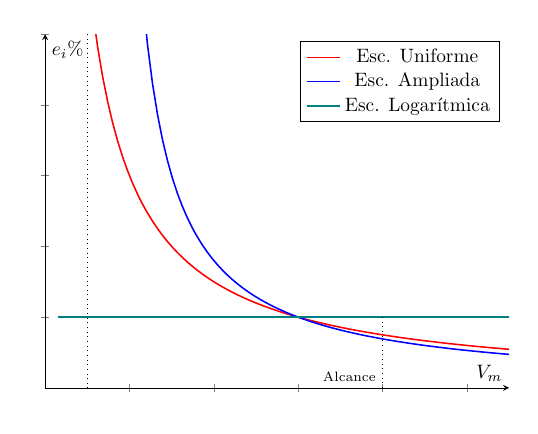
\begin{tikzpicture}[scale=0.7]
    \begin{axis}[
        axis lines = middle,
        xlabel = {$V_m$},
        ylabel = {$e_i\%$},
        domain = 0.3:12,
        ymin = 0, ymax = 10,
        xmin = 0, xmax = 11,
        samples = 100,
        width=10cm, height=8cm,
        restrict y to domain=0:12,
        xticklabel=\empty,
        yticklabel=\empty,
    ]
        \addplot [
            red,
            thick,
        ] {12/x};
        \addlegendentry{Esc. Uniforme}
        \addplot [
            blue,
            thick,
        ] {9/(x-1.5)};
        \addlegendentry{Esc. Ampliada}
        \addplot [
          teal,
          thick,
        ] {2};
        \addlegendentry{Esc. Logarítmica}

      \draw[black,dotted] (8,2) -- (8, 0) node[above left,black]{\scriptsize{Alcance}};
      \draw[black,dotted] (1,10) -- (1, 0);
    \end{axis}
  \end{tikzpicture}
  \caption{}
  \label{fig:error_no_lineal}
\end{figure}


\subsection{Propagación de errores (Mediciones Indirectas)}

Cuando una magnitud no se mide directamente, sino que se calcula a partir de otras mediciones (ej. Potencia \(P = V \cdot I\)), los errores de cada instrumento se propagan al resultado final.

Si una magnitud \(W\) depende de las variables \(X, Y, Z\), el error absoluto límite se obtiene mediante el diferencial total, adoptando el criterio pesimista (suma de valores absolutos):

\[
    E_W = \left| \frac{\partial W}{\partial X} \right| E_X + \left| \frac{\partial W}{\partial Y} \right| E_Y + \dots
\]

Sin embargo, para las operaciones más comunes en ingeniería (productos y cocientes), es mucho más práctico trabajar con el error relativo. Si \(W = X \cdot Y\) o \(W = X / Y\):

\begin{equation}
    e_W \approx e_X + e_Y
\end{equation}

Es decir, el error relativo total es la suma de los errores relativos de cada componente. Esto resalta nuevamente la importancia de medir en el tercio superior de la escala para minimizar los errores \(e_X\) y \(e_Y\) individuales antes de que se sumen.

\subsection{Análisis estadístico de los errores}

Una forma útil de minimizar los errores accidentales y garantizar una buena medida, es obtener varias mediciones de la misma magnitud, en las mismas condiciones, ya que es probable, en una serie de mediciones (de acuerdo a las leyes del azar), que exista una compensación de los errores accidentales.

Así, se pueden establecer tres postulados importantes;
\begin{enumerate}
  \item El valor verdadero de un número muy grande de mediciones efectuadas en las mismas condiciones, está dada por la media de los mismos.
  \item Es igualmente probable encontrar errores de igual valor absoluto pero de distinto signo.
  \item En una serie de mediciones, es tanto más probable cometer errores pequeños que grandes.
\end{enumerate}
